\begin{frame}{目录}
    \tableofcontents
\end{frame}

\section{最优策略和贝尔曼最优公式}

\begin{frame}{最优策略}
    状态价值可以用来评估一个策略的优劣。如果:
    \[
        v_{\pi_1}(s) \geq v_{\pi_2}(s), \forall s \in \mathcal{S}
    \]
    则称策略$\pi_1$优于策略$\pi_2$。
    \begin{block}{定义}
        若一个策略$\pi^*$对于所有的$s\in \mathcal{S}$和所有其他的策略$\pi$都满足$v_{\pi^*}(s)\geq v_\pi(s)$,则称$\pi^*$为最优策略。
    \end{block}
    \begin{itemize}
        \item 最优策略是否一定存在?
        \item 最优策略是否唯一?
        \item 最优策略是一个确定性策略还是一个随机策略?
        \item 如何得到最优策略?
    \end{itemize}
    使用\alert{贝尔曼最优公式}求解。
\end{frame}

\begin{frame}{贝尔曼最优公式}
    \textbf{贝尔曼最优公式}:
    \[
        \begin{aligned}
            v(s)&=\alert{\underset{\pi}{\max}}\sum_a\alert{\pi(a|s)}\left[\sum_r p(r|s,a)r+\gamma\sum_{s'}p(s'|s,a)v(s')\right], \quad \forall s\in\mathcal{S} \\
            &=\alert{\underset{\pi}{\max}}\sum_a\alert{\pi(a|s)}q(s,a), \quad \forall s\in\mathcal{S}
        \end{aligned}
    \]
    \begin{itemize}
        \item $p(r|s,a),p(s'|s,a),r,\gamma$都是已知的
        \item $v(s),v(s')$是未知的
        \item $\pi(s)$是已知还是未知的呢?
    \end{itemize}
\end{frame}

\begin{frame}{贝尔曼最优公式}
    \textbf{贝尔曼最优公式}:
    \[
        v(s)=\alert{\underset{\pi}{\max}}\sum_a\alert{\pi(a|s)}\left[\sum_r p(r|s,a)r+\gamma\sum_{s'}p(s'|s,a)v(s')\right], \quad \forall s\in\mathcal{S}
    \]
    \begin{examples}
        根据下述方程求解$x,a\in\mathbb{R}$:
        \[
            x=\underset{a}{\max}(2x-1-2a^2)
        \]
        先看式子的右半部分,无论$x$的取值如何,$\underset{a}{\max}(2x-1-2a^2)$的最大值都在$a=0$时取得,此时式子的右半部分为$2x-1$。然后再求解$x=2x-1$解得$x=1$。综上:$x=1,a=0$时原方程的解。
    \end{examples}
\end{frame}

\begin{frame}{贝尔曼最优公式}
    \textbf{贝尔曼最优公式}:
    \[
        \begin{aligned}
            v(s)&=\alert{\underset{\pi}{\max}}\sum_a\alert{\pi(a|s)}\left[\sum_r p(r|s,a)r+\gamma\sum_{s'}p(s'|s,a)v(s')\right], \quad \forall s\in\mathcal{S} \\
            &=\alert{\underset{\pi}{\max}}\sum_a\alert{\pi(a|s)}q(s,a) \\
            &=\alert{\underset{a\in\mathcal{A}(s)}{\max}q(s,a)}
        \end{aligned}
    \]
    当达到最优时,只需要让每次智能体都选择动作价值最大的行动即可,即:
    \[
        \pi(a|s)=
        \begin{cases}
            1 \quad a=a^* \\
            0 \quad a\neq a^*
        \end{cases}
    \]
    其中:
    \[
        a^*=\underset{a}{\arg\max} q(s,a)
    \]
\end{frame}

\begin{frame}{贝尔曼最优公式}
    确定了$\pi$之后,贝尔曼最优公式可以简化为:
    \[
        v=f(v)
    \]
    如何求解?
    \begin{theorem}
        对于任何具有$x=f(x)$形式的方程,如果$f$是一个\textit{压缩映射},那么:
        \begin{itemize}
            \item 解存在性:一定存在一个$x^*$满足$f(x^*)=x^*$
            \item 解唯一性:$x^*$是唯一的
            \item 求解方式(值迭代法):考虑一个数列$\{x_k\}$,其中$x_{k+1}=f(x_k)$。当$k\rightarrow\infty$时$x_k\rightarrow x^*$。
        \end{itemize}
    \end{theorem}
    贝尔曼最优公式是一个压缩映射(证明略)。
    \begin{itemize}
        \item 例:$x=0.5x$,$\{x_k\}=\{10, 5, 2.5,\cdots\}$
    \end{itemize}
\end{frame}

\begin{frame}{贝尔曼最优公式}
    所以我们可以按照值迭代法的求解方式求出$v^*$,但它一定就是最高的状态价值吗?
    \begin{theorem}
        假设$v^*$是$v=\max_\pi(r_\pi+P_\pi v)$的唯一解,那么对于任何其他给定策略$\pi$的满足$v_\pi=r_\pi+\gamma P_\pi v_\pi$的$v_\pi$而言都有:
        \[
            v^*\geq v_\pi \quad \forall \pi
        \]
    \end{theorem}
    也就是说,对于贝尔曼最优公式这一个特殊的方程,\alert{它的唯一解就是最优解!}
\end{frame}

\begin{frame}{贝尔曼最优公式}
    那么当状态价值取到最优的$v^*$时,策略$\pi^*$是什么样的呢?
    \[
        \alert{\pi^*(s)}=\arg\underset{\pi}{\max}\sum_a\pi(a|s)\left[\sum_r p(r|s,a)r+\gamma\sum_{s'}p(s'|s,a)\alert{v^*(s')}\right]
    \]
    \begin{theorem}
        对于任何$s\in \mathcal{S}$,下列确定性策略都是最优策略:
        \[
            \pi^*(a|s)=
            \begin{cases}
                1 \quad a=a^*(s) \\
                0 \quad a\neq a^*(s)
            \end{cases}
        \]
        其中:
        \[
                a^*(s)=\arg\underset{a}{\max} q^*(s,a),\quad
                q^*(s,a)=\sum_r p(r|s,a)r+\gamma\sum_{s'}p(s'|s,a)v^*(s')
        \]
    \end{theorem}

    也就是说,\alert{每次选择动作价值最高的动作就是最优策略!}
\end{frame}

\begin{frame}{值迭代法}
    奖励设置为:$r_{\text{boundary}}=r_{\text{forbidden}}=-1, r_{\text{target}}=1$。折扣系数为$\gamma=0.9$
    \begin{center}
        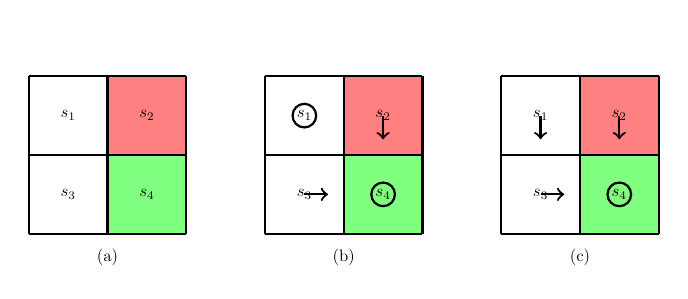
\begin{tikzpicture}
            % 填充指定格子为红色
            \fill[red!50] (1,1) rectangle (2,2); % 第2行第3列 (索引 (2,1))
            \fill[green!50] (1,0) rectangle (2,1); % 第3行第1列 (索引 (0,0))

            % 画3x3网格
            \draw[thick] (0,0) grid (2,2);
            
            % 标记状态编号 (行列索引)
            \foreach \x in {0,1,2} {
                \foreach \y in {0,1,2} {
                    \node at (\x+0.5, 2.5-\y){};
                }
            }
            
            % 绘制箭头表示策略
            % 示例:在格子中绘制箭头

           % 从 s_4 (0, 1) 向下
           \draw[thick] (0.5, 1.5) circle (0.15);

           % 从 s_5 (1, 1) 向右
           \draw[->, thick] (1.5, 1.5) -- (1.5, 1.2); % 向右


           % 从 s_7 (0, 2) 向右
           \draw[->, thick] (0.5, 0.5) -- (0.8, 0.5); % 向右

           % 从 s_9 (2, 2) 向左
           \draw[thick] (1.5, 0.5) circle (0.15);
            \node[scale=0.6] at (0.5, 1.5) {$s_1$};
            \node[scale=0.6] at (1.5, 1.5) {$s_2$};
            \node[scale=0.6] at (0.5, 0.5) {$s_3$};
            \node[scale=0.6] at (1.5, 0.5) {$s_4$};

            \node[scale=0.6] at (1, -0.3) {(b)};
            \node[scale=0.6] at (-2, -0.3) {(a)};
            \node[scale=0.6] at (4, -0.3) {(c)};

            % 填充指定格子为红色
            \fill[red!50] (-2,1) rectangle (-1,2); % 第2行第3列 (索引 (2,1))
            \fill[green!50] (-2,0) rectangle (-1,1); % 第3行第1列 (索引 (0,0))

            % 画3x3网格
            \draw[thick] (-3,0) grid (-1,2);
            
            % 标记状态编号 (行列索引)
            \foreach \x in {0,1,2} {
                \foreach \y in {0,1,2} {
                    \node at (\x+0.5, 2.5-\y){};
                }
            }
            
            % 绘制箭头表示策略
            % 示例:在格子中绘制箭头

           % 从 s_9 (2, 2) 向左
            \node[scale=0.6] at (-2.5, 1.5) {$s_1$};
            \node[scale=0.6] at (-1.5, 1.5) {$s_2$};
            \node[scale=0.6] at (-2.5, 0.5) {$s_3$};
            \node[scale=0.6] at (-1.5, 0.5) {$s_4$};

            % 填充指定格子为红色
            \fill[red!50] (4,1) rectangle (5,2); % 第2行第3列 (索引 (2,1))
            \fill[green!50] (4,0) rectangle (5,1); % 第3行第1列 (索引 (0,0))

            % 画3x3网格
            \draw[thick] (3,0) grid (5,2);
            
            % 标记状态编号 (行列索引)
            \foreach \x in {0,1,2} {
                \foreach \y in {0,1,2} {
                    \node at (\x+0.5, 2.5-\y){};
                }
            }
            
            % 绘制箭头表示策略
            % 示例:在格子中绘制箭头

           % 从 s_4 (0, 1) 向下
           \draw[->, thick] (3.5, 1.5) -- (3.5, 1.2); % 向下

           % 从 s_5 (1, 1) 向右
           \draw[->, thick] (4.5, 1.5) -- (4.5, 1.2); % 向右


           % 从 s_7 (0, 2) 向右
           \draw[->, thick] (3.5, 0.5) -- (3.8, 0.5); % 向右

           % 从 s_9 (2, 2) 向左
           \draw[thick] (4.5, 0.5) circle (0.15);
            \node[scale=0.6] at (3.5, 1.5) {$s_1$};
            \node[scale=0.6] at (4.5, 1.5) {$s_2$};
            \node[scale=0.6] at (3.5, 0.5) {$s_3$};
            \node[scale=0.6] at (4.5, 0.5) {$s_4$};
        \end{tikzpicture}
    \end{center}
    $q(s,a)$:
    \begin{table}[]
        \begin{tabular}{@{}cccccc@{}}
        \toprule
        动作价值    & $a_1$ & $a_2$ & $a_3$ & $a_4$ & $a_5$ \\ \midrule
        $s_1$ & $-1+\gamma v(s_1)$ & $-1+\gamma v(s_2)$ & $0+\gamma v(s_3)$ & $-1+\gamma v(s_1)$ & $0+\gamma v(s_1)$ \\
        $s_2$ & $-1+\gamma v(s_2)$ & $-1+\gamma v(s_2)$ & $1+\gamma v(s_4)$ & $0+\gamma v(s_1)$ & $-1+\gamma v(s_2)$ \\
        $s_3$ & $0+\gamma v(s_1)$ & $1+\gamma v(s_4)$ & $-1+\gamma v(s_3)$ & $-1+\gamma v(s_3)$ & $0+\gamma v(s_3)$ \\
        $s_4$ & $-1+\gamma v(s_2)$ & $-1+\gamma v(s_4)$ & $-1+\gamma v(s_4)$ & $0+\gamma v(s_3)$ & $1+\gamma v(s_4)$ \\ \bottomrule
        \end{tabular}
    \end{table}
\end{frame}

\begin{frame}{值迭代法}
    \begin{itemize}
        \item $k=0$:令$v_0(s_1)=v_0(s_2)=v_0(s_3)=v_0(s_4)=0$
        \begin{table}[]
            \begin{tabular}{@{}cccccc@{}}
            \toprule
            动作价值    & $a_1$ & $a_2$ & $a_3$ & $a_4$ & $a_5$ \\ \midrule
            $s_1$ & $-1$ & $-1$ & $\alert{0}$ & $-1$ & $\alert{0}$ \\
            $s_2$ & $-1$ & $-1$ & $\alert{1}$ & $0$ & $-1$ \\
            $s_3$ & $0$ & $\alert{1}$ & $-1$ & $-1$ & $0$ \\
            $s_4$ & $-1$ & $-1$ & $-1$ & $0$ & $\alert{1}$ \\ \bottomrule
            \end{tabular}
        \end{table}
    \end{itemize}
        第一步:策略更新
        \[
            \pi_1(a_5|s_1)=1, \pi_1(a_3|s_2)=1, \pi_1(a_2|s_3)=1, \pi_1(a_5|s_4)=1
        \]
        第二步:值更新
        \[
            v_1(s_1)=0,v_1(s_2)=1,v_1(s_3)=1,v_1(s_4)=1
        \]
        如图(b)所示。
\end{frame}

\begin{frame}{值迭代法}
    \begin{itemize}
        \item $k=1$:因为$v_1(s_1)=0,v_1(s_2)=1,v_1(s_3)=1,v_1(s_4)=1$,所以:
        \begin{table}[]
            \begin{tabular}{@{}cccccc@{}}
            \toprule
            动作价值    & $a_1$ & $a_2$ & $a_3$ & $a_4$ & $a_5$ \\ \midrule
            $s_1$ & $-1+\gamma 0$ & $-1+\gamma 1$ & $\alert{0+\gamma 1}$ & $-1+\gamma 0$ & $0+\gamma 0$ \\
            $s_2$ & $-1+\gamma 1$ & $-1+\gamma 1$ & $\alert{1+\gamma 1}$ & $0+\gamma 0$ & $-1+\gamma 1$ \\
            $s_3$ & $0+\gamma 0$ & $\alert{1+\gamma 1}$ & $-1+\gamma 1$ & $-1+\gamma 1$ & $0+\gamma 1$ \\
            $s_4$ & $-1+\gamma 1$ & $-1+\gamma 1$ & $-1+\gamma 1$ & $0+\gamma 1$ & $\alert{1+\gamma 1}$ \\ \bottomrule
            \end{tabular}
        \end{table}
    \end{itemize}
        第一步:策略更新
        \[
            \pi_1(a_3|s_1)=1, \pi_1(a_3|s_2)=1, \pi_1(a_2|s_3)=1, \pi_1(a_5|s_4)=1
        \]
        第二步:值更新
        \[
            v_2(s_1)=\gamma 1,v_2(s_2)=1+\gamma 1,v_2(s_3)=1+\gamma 1,v_2(s_4)=1+\gamma 1
        \]
        如图(c)所示(最优策略)
\end{frame}

\begin{frame}{小结}
    贝尔曼最优公式:
    \begin{itemize}
        \item 解存在性:根据压缩映射定理,一定存在解
        \item 解唯一性:根据压缩映射定理,解是唯一的
        \item 解最优性:根据最优策略定理,该解一定是最优解
        \item 求解方法:值迭代法
        \item 最优策略:最优状态价值对应的策略就是最优策略
    \end{itemize}
\end{frame}